\documentclass[12pt,a4paper]{article}
\usepackage[a4paper,top=12mm,bottom=14mm,left=15mm,right=15mm]{geometry}
\usepackage[T1]{fontenc}
\usepackage{amsmath}
\usepackage{amssymb}
\usepackage{enumitem}
\usepackage{xcolor}
\usepackage{tikz}
\usetikzlibrary{arrows.meta}

\pagestyle{empty}
\linespread{1.15}\selectfont
\setlength{\parskip}{5pt}
\setlength{\parindent}{0pt}

% ----------------------------------------------------------------
% Macros for the lattice multiplication grid (copied from the original)
\newcommand{\lsetup}[2]{%
  \edef\lC{\the\numexpr#1\relax}\edef\lR{\the\numexpr#2\relax}%
  \edef\lCm{\the\numexpr#1-1\relax}\edef\lRm{\the\numexpr#2-1\relax}}

\newcommand{\lgrid}{%
  \draw[thick] (0,0) rectangle (\lC,\lR);
  \foreach \i in {1,...,\lCm}{\draw (\i,0) -- (\i,\lR);}
  \foreach \j in {1,...,\lRm}{\draw (0,\j) -- (\lC,\j);}
  \foreach \i in {1,...,\lC}{\foreach \j in {1,...,\lR}{%
    \draw[gray!75] ({\i-1},{\j-1}) -- (\i,\j);}}}

\newcommand{\ltop}[2]{\node[font=\small] at ({#1-0.5},{\lR+0.34}) {#2};}
\newcommand{\lside}[2]{\node[font=\small] at ({\lC+0.34},{\lR-#1+0.5}) {#2};}

\newcommand{\lcell}[4]{%
  \node[font=\small] at ({#1-0.72},{\lR-#2+0.70}) {#3};
  \node[font=\small] at ({#1-0.28},{\lR-#2+0.30}) {#4};}

\newcommand{\lleft}[2]{\node[font=\small] at (-0.44,{\lR-#1+0.5}) {#2};}
\newcommand{\lbot}[2]{\node[font=\small] at ({#1-0.5},-0.42) {#2};}

\newcommand{\ltopdot}[1]{\fill (#1,{\lR+0.2}) circle (1.8pt);}
\newcommand{\lsidedot}[1]{\fill ({\lC+0.34},{\lR-#1}) circle (1.8pt);}

\newcommand{\lmeet}[2]{%
  \pgfmathsetmacro{\lmx}{#1}%
  \pgfmathsetmacro{\lmy}{\lR-#2}%
  \pgfmathsetmacro{\lts}{min(\lmx,\lmy)}%
  \pgfmathsetmacro{\lex}{\lmx-\lts}%
  \pgfmathsetmacro{\ley}{\lmy-\lts}%
  \pgfmathsetmacro{\ldx}{\lex<0.5 ? -0.44 : \lex}%
  \pgfmathsetmacro{\ldy}{\ley<0.5 ? -0.42 : \ley}}
\newcommand{\lansdot}[2]{\lmeet{#1}{#2}%
  \fill[red!75!black] ({\ldx},{\ldy}) circle (2.1pt);}
\newcommand{\ltrace}[2]{\lmeet{#1}{#2}%
  \draw[red!75!black,dashed,-{Stealth[length=2mm]}] ({\lmx},{\lR+0.1}) -- ({\lmx},{\lmy});
  \draw[red!75!black,dashed,-{Stealth[length=2mm]}] ({\lC+0.12},{\lmy}) -- ({\lmx},{\lmy});
  \ifdim\lts pt>0.1pt
    \draw[red!75!black,dashed,thick,-{Stealth[length=2mm]}] ({\lmx},{\lmy}) -- ({\lex},{\ley});
  \fi
  \fill[red!75!black] ({\ldx},{\ldy}) circle (2.1pt);}

\begin{document}

\begin{center}
  {\Large\bfseries Worked Solutions: The Lattice Multiplication Method}\\[6pt]
\end{center}

\section*{Q1. (a) $52\times34$}
The grid is already filled in. We add along the diagonals, starting from the bottom right corner.
\begin{center}
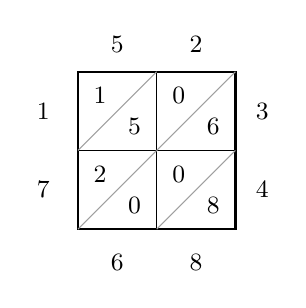
\begin{tikzpicture}[scale=1.0]
  \lsetup{2}{2}
  \lgrid
  \ltop{1}{5} \ltop{2}{2}
  \lside{1}{3} \lside{2}{4}
  \lcell{1}{1}{1}{5} \lcell{2}{1}{0}{6}
  \lcell{1}{2}{2}{0} \lcell{2}{2}{0}{8}
  \lleft{1}{1} \lleft{2}{7}
  \lbot{1}{6} \lbot{2}{8}
\end{tikzpicture}
\end{center}
Diagonals from bottom right:
\[
\begin{aligned}
\text{1st: } & 8 = 8,\\
\text{2nd: } & 0+0+6 = 6,\\
\text{3rd: } & 2+0+5 = 7,\\
\text{4th: } & 1 = 1.
\end{aligned}
\]
Reading the digits from left to right gives $1768$. So $52\times34=1768$.

\section*{Q1. (b) $68\times47$}
\begin{center}
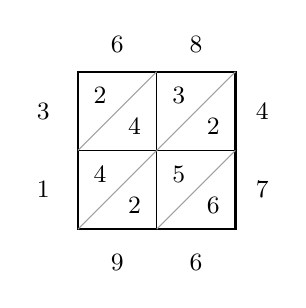
\begin{tikzpicture}[scale=1.0]
  \lsetup{2}{2}
  \lgrid
  \ltop{1}{6} \ltop{2}{8}
  \lside{1}{4} \lside{2}{7}
  \lcell{1}{1}{2}{4} \lcell{2}{1}{3}{2}
  \lcell{1}{2}{4}{2} \lcell{2}{2}{5}{6}
  \lleft{1}{3} \lleft{2}{1}
  \lbot{1}{9} \lbot{2}{6}
\end{tikzpicture}
\end{center}
Diagonals from bottom right:
\[
\begin{aligned}
\text{1st: } & 6 = 6,\\
\text{2nd: } & 5+2+2 = 9,\\
\text{3rd: } & 4+3+4 = 11 \quad \text{write } 1 \text{ and carry } 1,\\
\text{4th: } & 2+1 = 3.
\end{aligned}
\]
Reading the digits gives $3196$. So $68\times47=3196$.

\section*{Q2. (a) $34\times25$}
Fill the cells: $3\times2=06$, $4\times2=08$, $3\times5=15$, $4\times5=20$.
\begin{center}
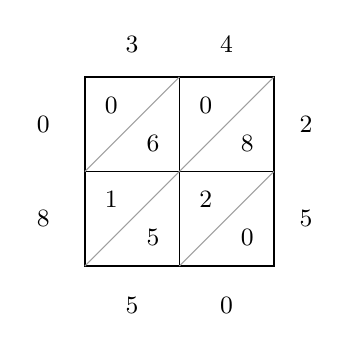
\begin{tikzpicture}[scale=1.2]
  \lsetup{2}{2}
  \lgrid
  \ltop{1}{3} \ltop{2}{4}
  \lside{1}{2} \lside{2}{5}
  \lcell{1}{1}{0}{6} \lcell{2}{1}{0}{8}
  \lcell{1}{2}{1}{5} \lcell{2}{2}{2}{0}
  \lleft{1}{0} \lleft{2}{8}
  \lbot{1}{5} \lbot{2}{0}
\end{tikzpicture}
\end{center}
Diagonals: $0$; $2+5+8=15$ so write $5$ carry $1$; $1+0+6+1=8$; $0$. The digits are $0850$, so $34\times25=850$.

\section*{Q2. (b) $243\times17$}
Fill the cells: $2\times1=02$, $4\times1=04$, $3\times1=03$, $2\times7=14$, $4\times7=28$, $3\times7=21$.
\begin{center}
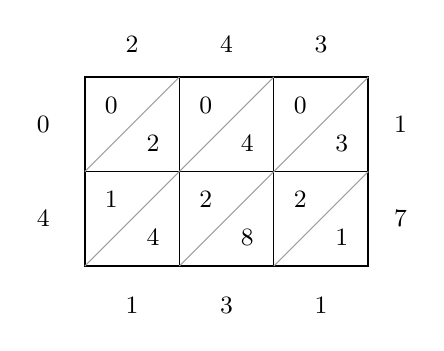
\begin{tikzpicture}[scale=1.2]
  \lsetup{3}{2}
  \lgrid
  \ltop{1}{2} \ltop{2}{4} \ltop{3}{3}
  \lside{1}{1} \lside{2}{7}
  \lcell{1}{1}{0}{2} \lcell{2}{1}{0}{4} \lcell{3}{1}{0}{3}
  \lcell{1}{2}{1}{4} \lcell{2}{2}{2}{8} \lcell{3}{2}{2}{1}
  \lleft{1}{0} \lleft{2}{4}
  \lbot{1}{1} \lbot{2}{3} \lbot{3}{1}
\end{tikzpicture}
\end{center}
Diagonals from bottom right: $1$; $2+8+3=13$ so write $3$ carry $1$; $2+4+4+0+1=11$ so write $1$ carry $1$; $1+0+2+1=4$; $0$. The digits are $04131$, so $243\times17=4131$.

\section*{Q3. $1.7\times4.3$}
\begin{center}
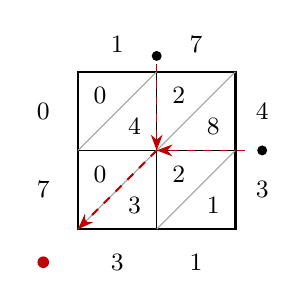
\begin{tikzpicture}[scale=1.0]
  \lsetup{2}{2}
  \lgrid
  \ltop{1}{1} \ltop{2}{7} \ltopdot{1}
  \lside{1}{4} \lside{2}{3} \lsidedot{1}
  \lcell{1}{1}{0}{4} \lcell{2}{1}{2}{8}
  \lcell{1}{2}{0}{3} \lcell{2}{2}{2}{1}
  \lleft{1}{0} \lleft{2}{7}
  \lbot{1}{3} \lbot{2}{1}
  \ltrace{1}{1}
\end{tikzpicture}
\end{center}
Diagonals: $1$; $2+3+8=13$ so write $3$ carry $1$; $0+2+4+1=7$; $0$. The digits are $0731$. The decimal point of $1.7$ is after the first column, and the decimal point of $4.3$ is after the first row. The two lines meet in the middle of the grid, and the diagonal leaves at the bottom left corner. So the point goes between the second and third digits: $07.31$. Hence $1.7\times4.3=7.31$.

\section*{Q4. (a) $0.6\times4.5$}
Fill the cells: $0\times4=00$, $6\times4=24$, $0\times5=00$, $6\times5=30$.
\begin{center}
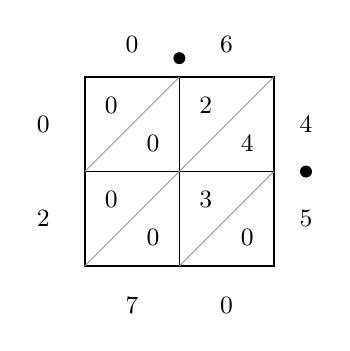
\begin{tikzpicture}[scale=1.2]
  \lsetup{2}{2}
  \lgrid
  \ltop{1}{0} \ltop{2}{6} \ltopdot{1}
  \lside{1}{4} \lside{2}{5} \lsidedot{1}
  \lcell{1}{1}{0}{0} \lcell{2}{1}{2}{4}
  \lcell{1}{2}{0}{0} \lcell{2}{2}{3}{0}
  \lleft{1}{0} \lleft{2}{2}
  \lbot{1}{7} \lbot{2}{0}
\end{tikzpicture}
\end{center}
Diagonals: $0$; $3+0+4=7$; $0+2+0=2$; $0$. The digits are $0270$. The decimal point is after the first column and first row, so the trace leaves at the bottom left corner. The point goes between the second and third digits: $02.70=2.7$. So $0.6\times4.5=2.7$.

\section*{Q4. (b) $12.4\times0.3$}
Fill the cells:
\begin{center}
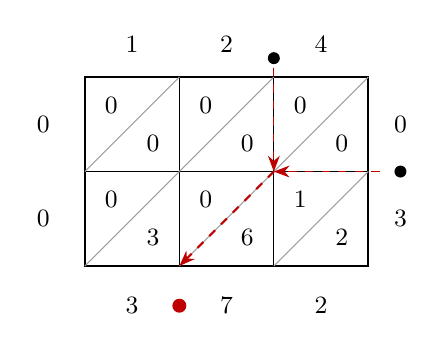
\begin{tikzpicture}[scale=1.2]
  \lsetup{3}{2}
  \lgrid
  \ltop{1}{1} \ltop{2}{2} \ltop{3}{4} \ltopdot{2}
  \lside{1}{0} \lside{2}{3} \lsidedot{1}
  \lcell{1}{1}{0}{0} \lcell{2}{1}{0}{0} \lcell{3}{1}{0}{0}
  \lcell{1}{2}{0}{3} \lcell{2}{2}{0}{6} \lcell{3}{2}{1}{2}
  \lleft{1}{0} \lleft{2}{0}
  \lbot{1}{3} \lbot{2}{7} \lbot{3}{2}
  \ltrace{2}{1}
\end{tikzpicture}
\end{center}
Diagonals: $2$; $1+6+0=7$; $0+3+0+0=3$; $0+0+0=0$; $0$. The digits are $00372$. The decimal point of $12.4$ is after the second column, and the decimal point of $0.3$ is after the first row. The lines meet one column in from the left, and the diagonal leaves through the bottom edge between the third and fourth digits. So the point goes between $3$ and $7$: $003.72=3.72$. So $12.4\times0.3=3.72$.

\section*{Q5.}
Using $0.6\times4.5=2.7$:
\begin{enumerate}[label=(\alph*)]
  \item $6\times45 = 270$. (Both numbers multiplied by $10$, so the answer is $100$ times larger.)
  \item $0.06\times4.5 = 0.27$. (The first number divided by $10$, so the answer is $10$ times smaller.)
  \item $60\times0.45 = 27$. (The first number multiplied by $100$, the second divided by $10$, so the answer is $10$ times larger.)
\end{enumerate}
The digits $27$ stay the same because the significant digits have not changed; only the place value changes.

\section*{Q6. (a) $24\times3.65$}
Fill the cells:
\begin{center}
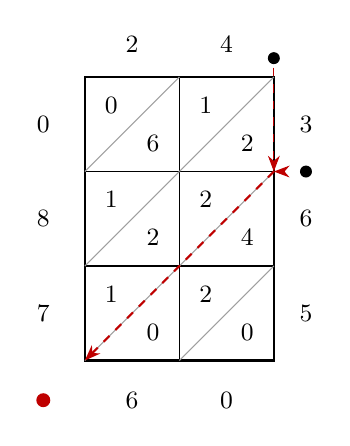
\begin{tikzpicture}[scale=1.2]
  \lsetup{2}{3}
  \lgrid
  \ltop{1}{2} \ltop{2}{4} \ltopdot{2}
  \lside{1}{3} \lside{2}{6} \lside{3}{5} \lsidedot{1}
  \lcell{1}{1}{0}{6} \lcell{2}{1}{1}{2}
  \lcell{1}{2}{1}{2} \lcell{2}{2}{2}{4}
  \lcell{1}{3}{1}{0} \lcell{2}{3}{2}{0}
  \lleft{1}{0} \lleft{2}{8} \lleft{3}{7}
  \lbot{1}{6} \lbot{2}{0}
  \ltrace{2}{1}
\end{tikzpicture}
\end{center}
Diagonals: $0$; $2+0+4=6$; $1+2+2+2=7$; $1+1+6=8$; $0$. The digits are $08760$. The decimal point of $24$ is on the right corner, and the decimal point of $3.65$ is after the first row. The trace leaves at the bottom left corner, so the point goes between the third and fourth digits: $087.60=87.60$. The order costs £$87.60$.

\section*{Q6. (b) $0.35\times16$}
Fill the cells:
\begin{center}
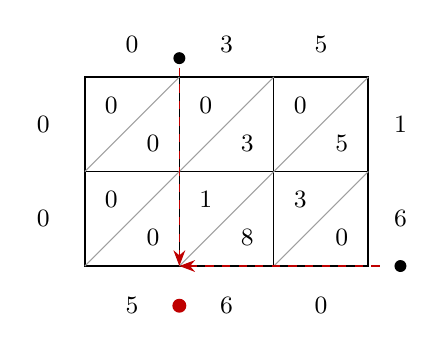
\begin{tikzpicture}[scale=1.2]
  \lsetup{3}{2}
  \lgrid
  \ltop{1}{0} \ltop{2}{3} \ltop{3}{5} \ltopdot{1}
  \lside{1}{1} \lside{2}{6} \lsidedot{2}
  \lcell{1}{1}{0}{0} \lcell{2}{1}{0}{3} \lcell{3}{1}{0}{5}
  \lcell{1}{2}{0}{0} \lcell{2}{2}{1}{8} \lcell{3}{2}{3}{0}
  \lleft{1}{0} \lleft{2}{0}
  \lbot{1}{5} \lbot{2}{6} \lbot{3}{0}
  \ltrace{1}{2}
\end{tikzpicture}
\end{center}
Diagonals: $0$; $3+8+5=16$ so write $6$ carry $1$; $1+0+3+0+1=5$; $0$; $0$. The digits are $00560$. The decimal point of $0.35$ is after the first column, and the decimal point of $16$ is on the bottom corner. The trace leaves through the bottom edge between the third and fourth digits, giving $005.60=5.60$. The tap loses $5.6$ litres.

\section*{Q7. (a) $1.45\times38$}
$1.45\times38 = 1.45\times(40-2) = 58 - 2.90 = 55.10$. Kofi pays £$55.10$.

\section*{Q7. (b) $4.8\times2.5$}
$4.8\times2.5 = 12.0$. The area is $12$ cm$^2$ (the trailing zero is not written).

\section*{Q8. Practice}
\begin{enumerate}[label=(\alph*)]
  \item $73\times48 = 3504$
  \item $5.2\times3.6 = 18.72$
  \item $0.9\times0.7 = 0.63$
  \item $126\times34 = 4284$
  \item $8.4\times0.25 = 2.1$
  \item $1.06\times3.5 = 3.71$
\end{enumerate}

\section*{Q9. Why the diagonals work}
\begin{enumerate}[label=(\alph*)]
  \item $40\times6 = 240$ and $7\times30 = 210$. Both are whole numbers of tens, so they both contribute to the tens column.
  \item In $47\times36$, the $4$ in $47$ really means $40$, and the $3$ in $36$ really means $30$. The cell for $4\times6$ represents $40\times6=240$, and the cell for $7\times3$ represents $7\times30=210$. Both products have the same place value (tens). Every cell on the same diagonal contributes to the same place value in the answer, so their digits are added together. This is why we add along diagonals, and why a total of $10$ or more carries into the next diagonal.
\end{enumerate}

\section*{Q10. $0.48\times0.25$}
\begin{enumerate}[label=(\alph*)]
  \item $0.48$ and $0.25$ are both less than $1$, so their product must be less than $1$. But $1200$ is greater than $1$, so it cannot be right.
  \item The correct product is $0.12$. 
  \begin{center}
  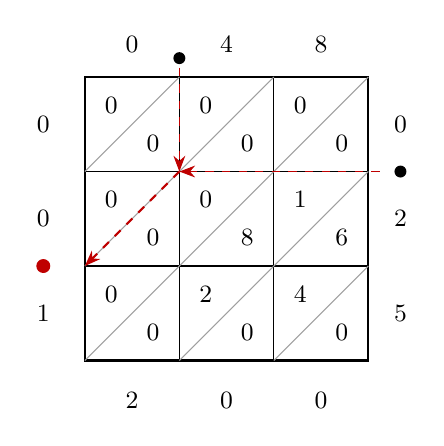
\begin{tikzpicture}[scale=1.2]
    \lsetup{3}{3}
    \lgrid
    \ltop{1}{0} \ltop{2}{4} \ltop{3}{8} \ltopdot{1}
    \lside{1}{0} \lside{2}{2} \lside{3}{5} \lsidedot{1}
    \lcell{1}{1}{0}{0} \lcell{2}{1}{0}{0} \lcell{3}{1}{0}{0}
    \lcell{1}{2}{0}{0} \lcell{2}{2}{0}{8} \lcell{3}{2}{1}{6}
    \lcell{1}{3}{0}{0} \lcell{2}{3}{2}{0} \lcell{3}{3}{4}{0}
    \lleft{1}{0} \lleft{2}{0} \lleft{3}{1}
    \lbot{1}{2} \lbot{2}{0} \lbot{3}{0}
    \ltrace{1}{1}
  \end{tikzpicture}
  \end{center}
  The diagonals give $0$; $4+0+6=10$ so write $0$ carry $1$; $2+1+0+8+0+1=12$ so write $2$ carry $1$; $0+0+0+0+0+1=1$; $0$; $0$. The digits are $001200$. The decimal point of $0.48$ is after the first column and the decimal point of $0.25$ is after the first row. The trace leaves through the left-hand side between the second and third digits, giving $00.1200=0.12$.
\end{enumerate}

\section*{Q11.}
A three-digit number has $3$ digits, and a four-digit number has $4$ digits. The grid has $3$ columns and $4$ rows, so it has $3\times4=12$ cells. Each cell needs one single-digit multiplication. So the method needs $12$ single-digit multiplications.

\section*{Q12.}
One example is $0.4\times0.9=0.36$. 
Using the lattice method with $04$ and $09$:
\begin{center}
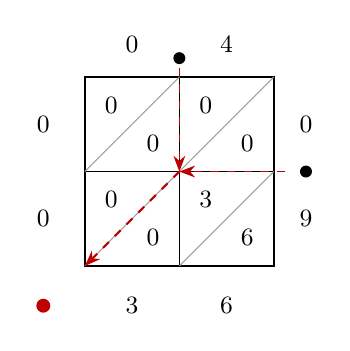
\begin{tikzpicture}[scale=1.2]
  \lsetup{2}{2}
  \lgrid
  \ltop{1}{0} \ltop{2}{4} \ltopdot{1}
  \lside{1}{0} \lside{2}{9} \lsidedot{1}
  \lcell{1}{1}{0}{0} \lcell{2}{1}{0}{0}
  \lcell{1}{2}{0}{0} \lcell{2}{2}{3}{6}
  \lleft{1}{0} \lleft{2}{0}
  \lbot{1}{3} \lbot{2}{6}
  \ltrace{1}{1}
\end{tikzpicture}
\end{center}
Diagonals: $6$; $3+0+0=3$; $0+0+0=0$; $0$. The digits are $0036$. Both decimal points are after the first column/row, so the point goes between the second and third digits: $00.36=0.36$. So $0.4\times0.9=0.36$.

\section*{Q13.}
Zainab is partly right. In the lattice method, you do not carry while filling in the grid, because each cell holds a single-digit multiplication and its two digits are written separately (tens above the diagonal, units below). However, you do carry when adding along the diagonals. For example, in Q1(b) $68\times47$, the third diagonal sum was $4+3+4=11$, so we had to write $1$ and carry $1$ into the next diagonal. So carrying still happens, just at the addition stage rather than during the multiplication.

\end{document}